% All-Pairs Shortest Paths: Floyd-Warshall -- Metropolis beamer slides
% Compile: pdflatex floyd-warshall.tex (x2)
\documentclass[10pt,aspectratio=169,xcolor=table]{beamer}

\usetheme{metropolis}
\metroset{block=fill, numbering=fraction, progressbar=frametitle}

\usepackage[T1]{fontenc}
\usepackage{amsmath, amssymb}
\usepackage{listings}
\usepackage{booktabs}
\usepackage{tikz}
\usetikzlibrary{arrows.meta, positioning, calc, decorations.pathmorphing}

% ---- colors -------------------------------------------------------------
\definecolor{mLightBlue}{HTML}{4C72B0}
\definecolor{mGreen}{HTML}{55A868}
\definecolor{mRed}{HTML}{C44E52}
\definecolor{mGray}{HTML}{BFBFBF}
\definecolor{mOrange}{HTML}{DD8452}
\setbeamercolor{alerted text}{fg=mRed}

% ---- code style ---------------------------------------------------------
\lstdefinestyle{jl}{
  basicstyle=\ttfamily\footnotesize,
  keywordstyle=\color{mRed}\bfseries,
  commentstyle=\color{mGreen}\itshape,
  numberstyle=\tiny\color{mGray},
  showstringspaces=false,
  breaklines=true,
  columns=fullflexible,
  morekeywords={function,for,in,if,else,elseif,end,return,length,while,continue,break}
}
\lstset{style=jl}

% ---- graph helpers ------------------------------------------------------
\tikzset{
  vtx/.style={draw, circle, minimum size=7mm, inner sep=0pt, font=\small,
              fill=white},
  edg/.style={thick, mGray!80!black},
  dedg/.style={edg, -{Stealth[length=2.5mm]}},
  hot/.style={line width=1.8pt, mLightBlue},
  wlbl/.style={fill=white, inner sep=1.5pt, font=\scriptsize, text=black},
  ok/.style={vtx, fill=mGreen!35},
  kk/.style={vtx, fill=mOrange!50},
}

% The running example. Arguments: styles for vertices 1, 2, 3, 4.
\newcommand{\fwgraph}[4]{%
  \begin{tikzpicture}[scale=0.85, every node/.append style={transform shape}]
    \node[#1] (1) at (0,0)      {1};
    \node[#2] (2) at (2.5,1.3)  {2};
    \node[#3] (3) at (2.5,-1.3) {3};
    \node[#4] (4) at (5,0)      {4};
    \draw[dedg] (1) -- node[wlbl] {10} (2);
    \draw[dedg] (1) -- node[wlbl] {5} (3);
    \draw[dedg] (2) -- node[wlbl] {2} (4);
    \draw[dedg] (3) -- node[wlbl] {3} (2);
    \draw[dedg] (3) -- node[wlbl] {1} (4);
    \draw[dedg] (4) .. controls (5,-2.9) and (0,-2.9) .. node[wlbl] {4} (1);
  \end{tikzpicture}%
}

% Matrix cells: \kc shades row/column k, \nw marks a value that just changed.
\newcommand{\kc}{\cellcolor{mOrange!20}}
\newcommand{\nw}[1]{\textcolor{mRed}{\textbf{#1}}}

% ---- title --------------------------------------------------------------
\title{All-Pairs Shortest Paths}
\subtitle{The Floyd-Warshall Algorithm}
\date{}
\author{}

\begin{document}

\maketitle

% =========================================================================
\begin{frame}{The Problem}
  Given a directed graph $G = (V, E)$ with edge weights $w(u, v)$, compute
  $\text{dist}(i, j)$ for \alert{every} pair of vertices $i, j$.

  \medskip
  The output is an $n \times n$ matrix $D$ with $D[i][j] = \text{dist}(i, j)$.

  \pause
  \bigskip
  First idea: run a single-source algorithm from every vertex.

  \medskip
  \begin{center}
  \begin{tabular}{llll}
    \toprule
    weights & run $n$ times & time & dense graph ($m \approx n^2$) \\
    \midrule
    unweighted & BFS & $O(n(n + m))$ & $O(n^3)$ \\
    $\ge 0$ & Dijkstra & $O(n(n + m) \log n)$ & $O(n^3 \log n)$ \\
    any & Bellman-Ford & $O(n^2 m)$ & $O(n^4)$ \\
    \bottomrule
  \end{tabular}
  \end{center}

  \pause
  \bigskip
  \alert{Floyd-Warshall}: any weights (no negative cycle), $O(n^3)$ time,
  and about ten lines of code.
\end{frame}

% =========================================================================
\section{The Recurrence}

\begin{frame}{Subproblems}
  Number the vertices $1, 2, \ldots, n$. The \alert{intermediate} vertices of
  a path are all its vertices except the two endpoints.

  \begin{block}{Definition}
    $D^{(k)}[i][j]$ = length of a shortest path from $i$ to $j$ whose
    intermediate vertices all lie in $\{1, 2, \ldots, k\}$.
  \end{block}

  \begin{center}
  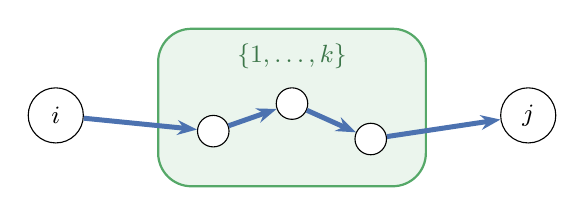
\begin{tikzpicture}
    \draw[mGreen, thick, fill=mGreen!12, rounded corners=12pt]
      (1.3,-0.9) rectangle (4.7,1.1);
    \node[mGreen!70!black, font=\small] at (3,0.75) {$\{1, \ldots, k\}$};
    \node[vtx] (i) at (0,0) {$i$};
    \node[vtx] (j) at (6,0) {$j$};
    \node[vtx, minimum size=4mm] (a) at (2,-0.2) {};
    \node[vtx, minimum size=4mm] (b) at (3,0.15) {};
    \node[vtx, minimum size=4mm] (c) at (4,-0.3) {};
    \draw[dedg, hot] (i) -- (a);
    \draw[dedg, hot] (a) -- (b);
    \draw[dedg, hot] (b) -- (c);
    \draw[dedg, hot] (c) -- (j);
  \end{tikzpicture}
  \end{center}

  \begin{itemize}
    \item $k = 0$: no intermediates, only direct edges.
    \item $k = n$: every vertex allowed, so $D^{(n)}[i][j] = \text{dist}(i, j)$.
  \end{itemize}
\end{frame}

\begin{frame}{Base Case}
  With no intermediate vertices, a path from $i$ to $j$ is either empty
  ($i = j$) or a single edge:
  \[
    D^{(0)}[i][j] =
    \begin{cases}
      0 & \text{if } i = j, \\
      w(i, j) & \text{if } (i, j) \in E, \\
      \infty & \text{otherwise.}
    \end{cases}
  \]

  \bigskip
  This is just the weighted adjacency matrix with zeros on the diagonal.
\end{frame}

\begin{frame}{The Recurrence}
  Now allow vertex $k$ as well. A shortest path from $i$ to $j$ with
  intermediates in $\{1, \ldots, k\}$ either

  \medskip
  \begin{columns}[t]
    \begin{column}{0.48\textwidth}
      \textbf{avoids $k$}
      \begin{center}
      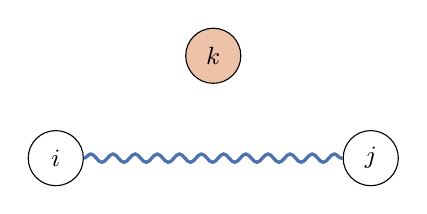
\begin{tikzpicture}
        \node[vtx] (i) at (0,0) {$i$};
        \node[vtx] (j) at (4,0) {$j$};
        \node[kk] (k) at (2,1.3) {$k$};
        \draw[very thick, mLightBlue, decorate,
              decoration={snake, amplitude=1.5pt, segment length=8pt}]
          (i) -- (j);
      \end{tikzpicture}
      \end{center}
      length $D^{(k-1)}[i][j]$
    \end{column}
    \begin{column}{0.48\textwidth}
      \textbf{goes through $k$}
      \begin{center}
      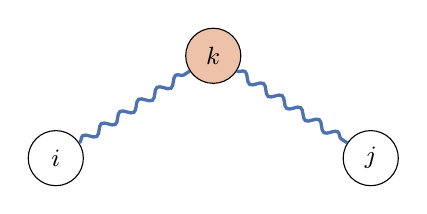
\begin{tikzpicture}
        \node[vtx] (i) at (0,0) {$i$};
        \node[vtx] (j) at (4,0) {$j$};
        \node[kk] (k) at (2,1.3) {$k$};
        \draw[very thick, mLightBlue, decorate,
              decoration={snake, amplitude=1.5pt, segment length=8pt}]
          (i) -- (k);
        \draw[very thick, mLightBlue, decorate,
              decoration={snake, amplitude=1.5pt, segment length=8pt}]
          (k) -- (j);
      \end{tikzpicture}
      \end{center}
      length $D^{(k-1)}[i][k] + D^{(k-1)}[k][j]$
    \end{column}
  \end{columns}

  \pause
  \bigskip
  \begin{block}{Recurrence}
    \[
      D^{(k)}[i][j] = \min\bigl(D^{(k-1)}[i][j],\;
                               D^{(k-1)}[i][k] + D^{(k-1)}[k][j]\bigr)
    \]
  \end{block}
\end{frame}

\begin{frame}{Why the Two Halves Use Only $\{1, \ldots, k - 1\}$}
  Suppose the path goes through $k$. With no negative cycle, we may assume it
  is \alert{simple}, so $k$ appears exactly once.

  \bigskip
  \begin{center}
  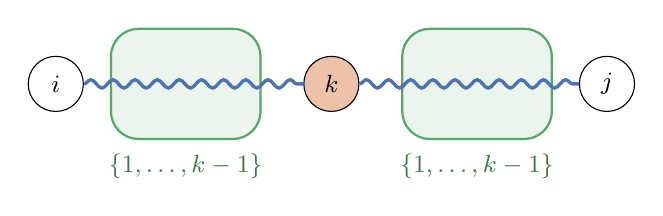
\begin{tikzpicture}
    \draw[mGreen, thick, fill=mGreen!12, rounded corners=10pt]
      (0.7,-0.7) rectangle (2.6,0.7);
    \draw[mGreen, thick, fill=mGreen!12, rounded corners=10pt]
      (4.4,-0.7) rectangle (6.3,0.7);
    \node[vtx] (i) at (0,0) {$i$};
    \node[kk] (k) at (3.5,0) {$k$};
    \node[vtx] (j) at (7,0) {$j$};
    \draw[very thick, mLightBlue, decorate,
          decoration={snake, amplitude=1.5pt, segment length=8pt}] (i) -- (k);
    \draw[very thick, mLightBlue, decorate,
          decoration={snake, amplitude=1.5pt, segment length=8pt}] (k) -- (j);
    \node[mGreen!70!black, font=\small] at (1.65,-1.05) {$\{1, \ldots, k-1\}$};
    \node[mGreen!70!black, font=\small] at (5.35,-1.05) {$\{1, \ldots, k-1\}$};
  \end{tikzpicture}
  \end{center}

  \bigskip
  \begin{itemize}
    \item The part $i \leadsto k$ has $k$ as an endpoint, not an intermediate.
          The same holds for $k \leadsto j$.
    \item Each part must itself be shortest among such paths, so they have
          lengths $D^{(k-1)}[i][k]$ and $D^{(k-1)}[k][j]$.
  \end{itemize}
\end{frame}

% =========================================================================
\section{The Algorithm}

\begin{frame}[fragile]{Floyd-Warshall}
  \begin{columns}[c]
    \begin{column}{0.5\textwidth}
\begin{lstlisting}
function floyd_warshall(n, W)
    D = copy(W)  # D^(0)
    for k in 1:n
        for i in 1:n
            for j in 1:n
                if D[i,k] + D[k,j] < D[i,j]
                    D[i,j] = D[i,k] + D[k,j]
                end
            end
        end
    end
    return D
end
\end{lstlisting}
    \end{column}
    \begin{column}{0.45\textwidth}
      \begin{itemize}
        \item The outer loop must be over $k$: $D^{(k)}$ needs all of
              $D^{(k-1)}$.
        \item One matrix, updated \alert{in place}, instead of $n + 1$
              matrices.
        \item Time $O(n^3)$, space $O(n^2)$.
      \end{itemize}
    \end{column}
  \end{columns}
\end{frame}

\begin{frame}{Why Updating in Place Is Safe}
  In round $k$ we read $D[i][k]$ and $D[k][j]$ while possibly overwriting
  other entries. Do these two entries change during round $k$?

  \pause
  \bigskip
  \begin{itemize}
    \item The update for entry $[i][k]$ is
          \[
            D[i][k] \gets \min\bigl(D[i][k],\; D[i][k] + D[k][k]\bigr).
          \]
    \item $D[k][k] = 0$ unless there is a negative cycle through $k$.
    \item So $D[i][k]$ stays the same, and likewise $D[k][j]$.
  \end{itemize}

  \bigskip
  Row $k$ and column $k$ are fixed during round $k$, so it does not matter
  whether we read old or new values elsewhere.
\end{frame}

% =========================================================================
\section{Example}

\begin{frame}{Example: $D^{(0)}$}
  \begin{columns}[c]
    \begin{column}{0.48\textwidth}
      \begin{center}\fwgraph{vtx}{vtx}{vtx}{vtx}\end{center}
    \end{column}
    \begin{column}{0.48\textwidth}
      \begin{center}
      \renewcommand{\arraystretch}{1.3}
      \begin{tabular}{c|cccc}
            & 1 & 2 & 3 & 4 \\ \hline
        1 & 0 & 10 & 5 & $\infty$ \\
        2 & $\infty$ & 0 & $\infty$ & 2 \\
        3 & $\infty$ & 3 & 0 & 1 \\
        4 & 4 & $\infty$ & $\infty$ & 0 \\
      \end{tabular}
      \end{center}

      \medskip
      \small Direct edges only.
    \end{column}
  \end{columns}
\end{frame}

\begin{frame}{Example: $D^{(1)}$, through vertex 1}
  \begin{columns}[c]
    \begin{column}{0.48\textwidth}
      \begin{center}\fwgraph{kk}{vtx}{vtx}{vtx}\end{center}
    \end{column}
    \begin{column}{0.48\textwidth}
      \begin{center}
      \renewcommand{\arraystretch}{1.3}
      \begin{tabular}{c|cccc}
            & 1 & 2 & 3 & 4 \\ \hline
        1 & \kc 0 & \kc 10 & \kc 5 & \kc $\infty$ \\
        2 & \kc $\infty$ & 0 & $\infty$ & 2 \\
        3 & \kc $\infty$ & 3 & 0 & 1 \\
        4 & \kc 4 & \nw{14} & \nw{9} & 0 \\
      \end{tabular}
      \end{center}

      \medskip
      \small Only vertex 4 has an edge into 1.\\
      $D[4][2] = 4 + 10 = 14$, \quad $D[4][3] = 4 + 5 = 9$.
    \end{column}
  \end{columns}
\end{frame}

\begin{frame}{Example: $D^{(2)}$, through vertices 1, 2}
  \begin{columns}[c]
    \begin{column}{0.48\textwidth}
      \begin{center}\fwgraph{ok}{kk}{vtx}{vtx}\end{center}
    \end{column}
    \begin{column}{0.48\textwidth}
      \begin{center}
      \renewcommand{\arraystretch}{1.3}
      \begin{tabular}{c|cccc}
            & 1 & 2 & 3 & 4 \\ \hline
        1 & 0 & \kc 10 & 5 & \nw{12} \\
        2 & \kc $\infty$ & \kc 0 & \kc $\infty$ & \kc 2 \\
        3 & $\infty$ & \kc 3 & 0 & 1 \\
        4 & 4 & \kc 14 & 9 & 0 \\
      \end{tabular}
      \end{center}

      \medskip
      \small Vertex 2 only leads to 4.\\
      $D[1][4] = 10 + 2 = 12$.\\
      ($D[3][4]$: $3 + 2 = 5$ does not beat $1$.)
    \end{column}
  \end{columns}
\end{frame}

\begin{frame}{Example: $D^{(3)}$, through vertices 1, 2, 3}
  \begin{columns}[c]
    \begin{column}{0.48\textwidth}
      \begin{center}\fwgraph{ok}{ok}{kk}{vtx}\end{center}
    \end{column}
    \begin{column}{0.48\textwidth}
      \begin{center}
      \renewcommand{\arraystretch}{1.3}
      \begin{tabular}{c|cccc}
            & 1 & 2 & 3 & 4 \\ \hline
        1 & 0 & \nw{8} & \kc 5 & \nw{6} \\
        2 & $\infty$ & 0 & \kc $\infty$ & 2 \\
        3 & \kc $\infty$ & \kc 3 & \kc 0 & \kc 1 \\
        4 & 4 & \nw{12} & \kc 9 & 0 \\
      \end{tabular}
      \end{center}

      \medskip
      \small $D[1][2] = 5 + 3 = 8$, \quad $D[1][4] = 5 + 1 = 6$,\\
      $D[4][2] = 9 + 3 = 12$.
    \end{column}
  \end{columns}
\end{frame}

\begin{frame}{Example: $D^{(4)}$, every vertex allowed}
  \begin{columns}[c]
    \begin{column}{0.48\textwidth}
      \begin{center}\fwgraph{ok}{ok}{ok}{kk}\end{center}
    \end{column}
    \begin{column}{0.48\textwidth}
      \begin{center}
      \renewcommand{\arraystretch}{1.3}
      \begin{tabular}{c|cccc}
            & 1 & 2 & 3 & 4 \\ \hline
        1 & 0 & 8 & 5 & \kc 6 \\
        2 & \nw{6} & 0 & \nw{11} & \kc 2 \\
        3 & \nw{5} & 3 & 0 & \kc 1 \\
        4 & \kc 4 & \kc 12 & \kc 9 & \kc 0 \\
      \end{tabular}
      \end{center}

      \medskip
      \small The edge $4 \to 1$ finally lets 2 and 3 reach 1.\\
      $D[2][1] = 2 + 4 = 6$, \quad $D[2][3] = 2 + 9 = 11$,\\
      $D[3][1] = 1 + 4 = 5$.
    \end{column}
  \end{columns}
\end{frame}

% =========================================================================
\section{Correctness and Extensions}

\begin{frame}{Correctness}
  \begin{block}{Claim}
    After round $k$, $D[i][j] = D^{(k)}[i][j]$ for all $i, j$.
  \end{block}

  \medskip
  \textbf{Proof} by induction on $k$.
  \begin{itemize}
    \item $k = 0$: $D$ starts as $D^{(0)}$ by construction.
    \item $k \ge 1$: assume $D = D^{(k-1)}$ before round $k$. Row $k$ and
          column $k$ do not change during the round, so each update computes
          \[
            \min\bigl(D^{(k-1)}[i][j],\; D^{(k-1)}[i][k] + D^{(k-1)}[k][j]\bigr),
          \]
          which is $D^{(k)}[i][j]$ by the recurrence.
  \end{itemize}

  \medskip
  With $k = n$ every vertex may be an intermediate, so $D[i][j] =
  \text{dist}(i, j)$. \hfill $\square$
\end{frame}

\begin{frame}{Recovering the Paths}
  Keep a second matrix $P[i][j]$ = the vertex just \alert{before} $j$ on the
  best path from $i$ to $j$ found so far.

  \begin{itemize}
    \item Start: $P[i][j] = i$ if $(i, j) \in E$, otherwise undefined.
    \item When the path through $k$ wins: $P[i][j] \gets P[k][j]$, since the
          path now ends the same way as the best path from $k$ to $j$.
  \end{itemize}

  \pause
  \medskip
  To print the path from $i$ to $j$, follow $P$ backwards from $j$:
  \[
    j,\; P[i][j],\; P[i][P[i][j]],\; \ldots,\; i.
  \]

  \pause
  \textbf{Example} ($4 \to 2$, length 12):
  $P[4][2] = 3$, $P[4][3] = 1$, $P[4][1] = 4$. \\
  So the path is $4 \to 1 \to 3 \to 2$, with length $4 + 5 + 3 = 12$.
\end{frame}

\begin{frame}{Detecting Negative Cycles}
  Floyd-Warshall assumes there is no negative cycle. If there is one, it
  shows up on the \alert{diagonal}.

  \bigskip
  \begin{itemize}
    \item Every value $D[i][i]$ is the length of some closed walk through $i$,
          so $D[i][i] < 0$ means there is a negative cycle.
    \item Conversely, let $C$ be a negative cycle, $k$ its largest vertex and
          $i \ne k$ another vertex of $C$. The two arcs of $C$ between $i$ and
          $k$ use only intermediates below $k$, so after round $k$,
          $D[i][i] \le \text{length}(C) < 0$.
  \end{itemize}

  \begin{block}{Check}
    After the algorithm finishes: there is a negative cycle
    $\iff$ $D[i][i] < 0$ for some $i$.
  \end{block}
\end{frame}

\begin{frame}[fragile]{Floyd-Warshall in Julia}
  \begin{columns}[c]
    \begin{column}{0.55\textwidth}
\begin{lstlisting}[basicstyle=\ttfamily\scriptsize]
# W[i,j] = edge weight, Inf if no edge, 0 on the diagonal
function floyd_warshall(W)
    n = size(W, 1)
    D = copy(W)
    for k in 1:n
        for i in 1:n
            D[i,k] == Inf && continue   # nothing to gain
            for j in 1:n
                if D[i,k] + D[k,j] < D[i,j]
                    D[i,j] = D[i,k] + D[k,j]
                end
            end
        end
    end
    for i in 1:n
        D[i,i] < 0 && error("negative cycle detected")
    end
    return D
end
\end{lstlisting}
    \end{column}
    \begin{column}{0.4\textwidth}
      \begin{itemize}
        \item \texttt{D} is an $n \times n$ matrix, indexed
              \texttt{D[i,j]}.
        \item Skipping rows with \texttt{D[i,k] == Inf} avoids pointless
              work on sparse graphs.
      \end{itemize}
    \end{column}
  \end{columns}
\end{frame}

% =========================================================================
\begin{frame}{Exercise}
  \begin{columns}[c]
    \begin{column}{0.4\textwidth}
      \begin{center}
      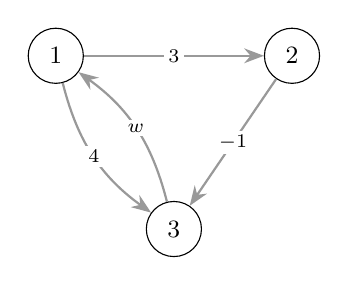
\begin{tikzpicture}
        \node[vtx] (1) at (0,0) {1};
        \node[vtx] (2) at (3,0) {2};
        \node[vtx] (3) at (1.5,-2.2) {3};
        \draw[dedg] (1) -- node[wlbl] {3} (2);
        \draw[dedg] (2) -- node[wlbl] {$-1$} (3);
        \draw[dedg] (1) to[bend right=20] node[wlbl] {4} (3);
        \draw[dedg] (3) to[bend right=20] node[wlbl] {$w$} (1);
      \end{tikzpicture}
      \end{center}
    \end{column}
    \begin{column}{0.55\textwidth}
      \begin{enumerate}
        \item Take $w = 2$. Write down $D^{(0)}$, then run Floyd-Warshall
              and give $D^{(1)}, D^{(2)}, D^{(3)}$.
        \item Now take $w = -3$. What does the algorithm report, and why?
      \end{enumerate}
    \end{column}
  \end{columns}
\end{frame}

\begin{frame}{Solution}
  \small
  \textbf{(a)} $w = 2$:

  \medskip
  \begin{center}
  \renewcommand{\arraystretch}{1.2}
  \begin{tabular}{c|ccc}
      $D^{(0)}$ & 1 & 2 & 3 \\ \hline
    1 & 0 & 3 & 4 \\
    2 & $\infty$ & 0 & $-1$ \\
    3 & 2 & $\infty$ & 0 \\
  \end{tabular}
  \quad
  \begin{tabular}{c|ccc}
      $D^{(1)}$ & 1 & 2 & 3 \\ \hline
    1 & 0 & 3 & 4 \\
    2 & $\infty$ & 0 & $-1$ \\
    3 & 2 & \nw{5} & 0 \\
  \end{tabular}
  \quad
  \begin{tabular}{c|ccc}
      $D^{(2)}$ & 1 & 2 & 3 \\ \hline
    1 & 0 & 3 & \nw{2} \\
    2 & $\infty$ & 0 & $-1$ \\
    3 & 2 & 5 & 0 \\
  \end{tabular}
  \quad
  \begin{tabular}{c|ccc}
      $D^{(3)}$ & 1 & 2 & 3 \\ \hline
    1 & 0 & 3 & 2 \\
    2 & \nw{1} & 0 & $-1$ \\
    3 & 2 & 5 & 0 \\
  \end{tabular}
  \end{center}

  \medskip
  For example $D[1][3] = 3 + (-1) = 2$ goes through 2, beating the direct
  edge of weight 4, and $D[2][1] = -1 + 2 = 1$ goes through 3.

  \pause
  \bigskip
  \textbf{(b)} $w = -3$: the cycle $1 \to 2 \to 3 \to 1$ has length
  $3 - 1 - 3 = -1 < 0$. The final matrix has $D[1][1] = -1$ (and
  $D[2][2] = -1$, $D[3][3] = -2$), so the algorithm reports a negative
  cycle. The other entries are meaningless, since no shortest paths exist.
\end{frame}

% =========================================================================
\begin{frame}{Summary}
  \begin{itemize}
    \item $D^{(k)}[i][j]$: shortest $i \to j$ path whose intermediates lie in
          $\{1, \ldots, k\}$.
    \item Recurrence: either avoid $k$, or go $i \leadsto k \leadsto j$.
    \item Three nested loops with $k$ outermost, one matrix updated in place.
    \item $O(n^3)$ time, $O(n^2)$ space, negative edges allowed.
    \item A negative entry on the diagonal reveals a negative cycle.
  \end{itemize}

  \bigskip
  \begin{center}
  \begin{tabular}{lll}
    \toprule
    situation & best choice & time \\
    \midrule
    sparse, weights $\ge 0$ & Dijkstra from each vertex & $O(nm \log n)$ \\
    dense, or negative weights & Floyd-Warshall & $O(n^3)$ \\
    \bottomrule
  \end{tabular}
  \end{center}
\end{frame}

\end{document}
